% !TEX program = lualatex
\documentclass[11pt,a5paper]{article}

% -------- LuaLaTeX : polices et langue --------
\usepackage{fontspec}
\setmainfont{Latin Modern Roman}
\setsansfont{Tex Gyre Heros}
\renewcommand{\familydefault}{\sfdefault} % force le sans serif par défaut
\usepackage{polyglossia}
\setdefaultlanguage{french}

% -------- Mise en page --------
\usepackage[a5paper,margin=1cm]{geometry}
\usepackage{multicol}
\usepackage{fancyhdr}
\pagestyle{empty}
\usepackage{enumitem}
\usepackage{array}
\usepackage{amssymb}  % \square
\usepackage{xcolor}
\usepackage{microtype}
\usepackage{tabularx}
\newcolumntype{Y}{>{\centering\arraybackslash}X}
\usepackage{graphicx} % indispensable pour \includegraphics

% Styles
\setlist[itemize]{leftmargin=1.2em}
\setlist[enumerate]{nosep,leftmargin=1.6em}
\setlength{\parskip}{0.4em}
\setlength{\parindent}{0pt}

% Cases à cocher
\newcommand{\checkbox}{\(\square\)}
\newcommand{\choix}[1]{\checkbox\ #1}
\newcommand{\ligne}{{\color{gray!60}\hrulefill}}
\begin{document}

\begin{center}
\LARGE\textbf{Calendrier de l’année 2025−2026}
\end{center}

% T1
\section*{Trimestre 1}
\begin{itemize}
  \item recherche du lieu de stage \ligne
  \item réunion parents / professeurs \ligne
\end{itemize}

% T2
\section*{Trimestre 2}
\begin{itemize}
  \item brevet blanc n°1 \ligne
  \item stage d'observation en entreprise \ligne
  \item rapport de stage à rendre \ligne
  \item forum des métiers et formations \ligne
  \item Journées Portes Ouvertes des établissements \ligne
\end{itemize}

% T3
\section*{Trimestre 3}
\begin{itemize}[itemsep=0.2em]
  \item brevet blanc n°2 \ligne
  \item oral blanc \ligne
  \item vœux d'orientations \ligne
  \item épreuve orale officielle du DNB \ligne
  \item épreuves écrites officielles du DNB \ligne
  \item résultats d’affectations \ligne
\end{itemize}

\section*{Toute l’année}
\textbf{RDV orientation avec Mme Ithier} \ligne \\
Conseillère d'Orientation, Psychologue de l'Éducation Nationale\\
\emph{(prise de rendez-vous en vie scolaire)}

\newpage
Prénom et nom : \ligne

% Projet métier
\section*{Projet et centres d'intérêt}

Idée/envie du métier que je souhaite exercer plus tard :

\ligne

\vspace{0.6em}
Je coche trois domaines qui pourraient me correspondre :

\begin{multicols}{3}
\begin{itemize}[label=\checkbox]
  \item nature
  \item arts
  \item communication
  \item soin aux personnes
  \item animaux
  \item construction
  \item agriculture
  \item médical
  \item technologies
  \item culture
  \item environnement
  \item transports
  \item alimentation
  \item informatique
  \item services
  \item restauration
  \item réparation
  \item médias
  \item tourisme
  \item police
  \item sport
  \item sécurité
  \item vente et hôtellerie
  \item beauté
  \item enfants
  \item fabrication
  \item logistique
  \item justice
  \item langues étrangères
  \item éducation
  \item design
  \item conseil
  \item économie
  \item ingénérie
  \item commerce
  \item langues
\end{itemize}

\end{multicols}

\vspace{0.6em}
% Intérêt pour les matières
Intérêt pour les matières, indépendemment de mes résultats :

\newcommand{\avis}{\hfill \(\square\ \square\ \square\ \square\ \square\)}
\begin{itemize}[topsep=0pt]
  \item Anglais, Espagnol \avis
  \item Français, Histoire Géographie \avis
  \item Mathématiques, Sciences Physiques, SVT, Technologie \avis
  \item Éducation Musicale, Arts plastiques \avis
  \item Éducation Physique et Sportive \avis
\end{itemize}
\newpage
J'ai bien compris les trois possibilités, et surtout les différences entre elles, après la troisième : 2de GT, 2de Pro et Apprentissage.

\vspace{0.6em}
\begin{tabularx}{\textwidth}{Y Y Y}
\choix{Oui} & \choix{Pas complètement} & \choix{Non}
\end{tabularx}

\vspace{1.6em}
Idée/envie pour mon premier vœu en fin d'année :

\vspace{0.4em}
\begin{tabularx}{\textwidth}{Y | Y Y}
\choix{2de GT} & \choix{2de Pro} & \choix{Apprentissage}\\
[0.4em]
& \multicolumn{2}{c}{Métier / famille : \ligne }
\end{tabularx}
\begin{center}
\choix{Ne sait pas pour l'instant}
\end{center}

% Études et ressenti
\section*{Études et ressenti}

J'envisage des études ...

\begin{itemize}[label=\square, topsep=0pt]
\item le plus courtes possibles
\item jusqu'au bac (3 ans après le collège)
\item supérieures (2, 3, 5, 8 … ans après le bac)
\end{itemize}


\vspace{1.2em}
Par rapport à mon orientation en fin d'année, je me sens concerné(e)/impliqué(e) …
\begin{itemize}[label=\square, topsep=0pt]
\item pas du tout
\item « normalement »
\item beaucoup
\end{itemize}


\vspace{1.2em}
Cela me stresse / m'inquiète …
\begin{itemize}[label=\square, topsep=0pt]
\item pas du tout
\item un peu
\item beaucoup
\end{itemize}

\newpage
\begin{center}
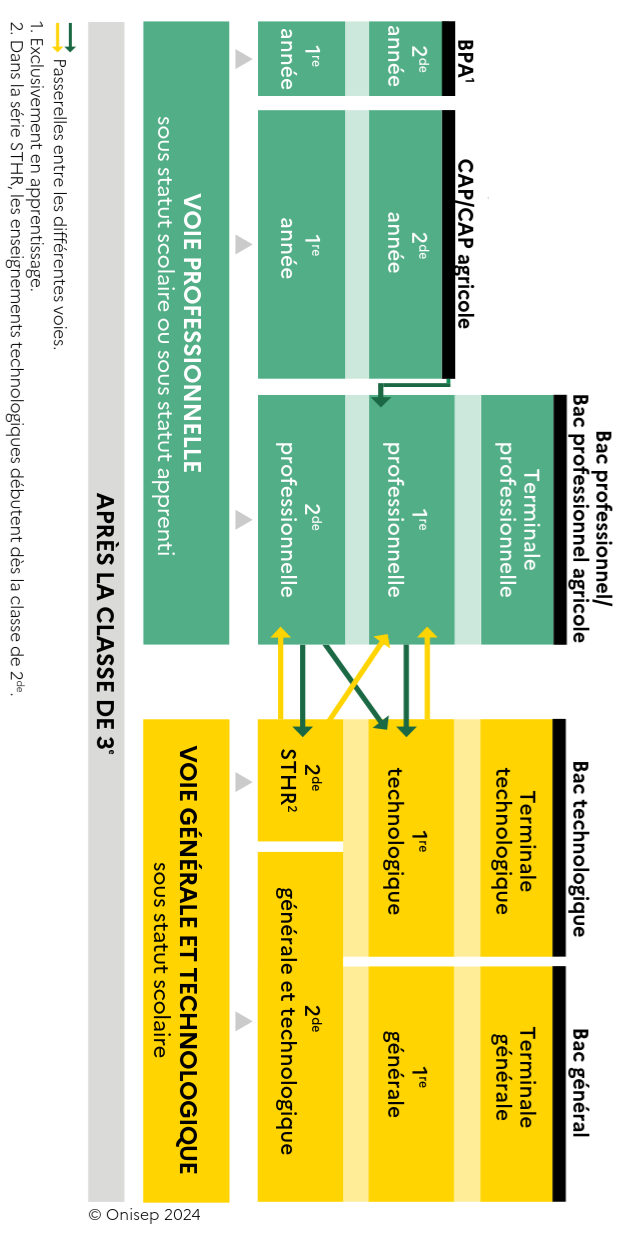
\includegraphics[width=0.75\textwidth]{images/orientation-apres-troisieme.png}
\end{center}


\end{document}
